\documentclass[12pt, letterpaper]{article}

\usepackage[utf8]{inputenc}
\usepackage[english]{babel}
\usepackage[T1]{fontenc}
\usepackage{graphicx}
\usepackage{tikz}
\usepackage{subfig}
\usepackage{wrapfig}
\usepackage{longtable}
\usepackage{amsmath}
\newcommand\tab[1][1cm]{\hspace*{#1}}
\renewcommand{\baselinestretch}{1.3}

\begin{document}

\begin{titlepage}

\begin{center}
	\large{EC336: Embedded Systems}\\
	\huge{\textbf{Interfacing ADC and DAC}}\\
	\large{Arvind S Kumar (15EC106), Pavan M (15EC137),\\ Samarth B (15EC143), Sripathi M (15EC149)}\\
	\large{31 August 2018}
\end{center}	

\begin{figure}[!h]
	\centering
	
\includegraphics[scale=0.8]{NITKEmblem.png}
	\label{fig:NITKEmblem}
\end{figure}	
\begin{center}
	
\huge{Submitted to:}\\
\begin{large}
Prof. Ramesh Kini M, Prof. Arulalan Rajan\\
Department of Electronics and Communication Engineering\\
NITK, Surathkal
\end{large}

\end{center}

\end{titlepage}

\section{Goal of the Lab}

The aim of this lab was to interface the inbuilt ADC and external DAC  with the microcontroller chip. The board chosen by our group for this exercise was Texas Instruments' MSP430G2553 launchpad.

\section{Components Used}

For this lab the components used are :

\begin{itemize}
	\item MSP430 microcontroller
	\item LEDs
	\item 220 $\Omega$ resistors
	\item DAC0808 IC 
	\item Op-amp IC $\nu$A741
	\item Capacitors 1 $\nu$F
\end{itemize}

\section{Board Details}

Some of the features of the MSP430 are - (Refer Figure \ref{fig:architecture} and Figure \ref{fig:board} for more information)

\begin{itemize}
	\item 16-bit RISC architecture
	\item Von-Neumann architecture
	\item Upto 16 MHz clock frequency
	\item Low power consumption and five power saving modes
	\item 16 general purpose registers
	\item 10-bit ADC
	\item Supports SPI, I2C, UART and USB interfaces
	\item Has 16 GPIO pins divided as two ports (8-bit each)
\end{itemize}
	
\begin{figure}[t]
	\centering
	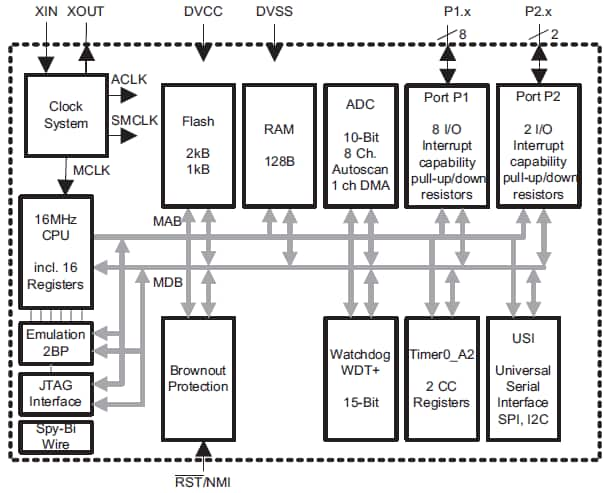
\includegraphics[scale=0.8]{msp430g2231-ep-ti.png}
	\caption{MSP430 Architecture}
	\label{fig:architecture}
\end{figure}

\begin{figure}[t]
	\centering
	\subfloat[fig:board][Board]{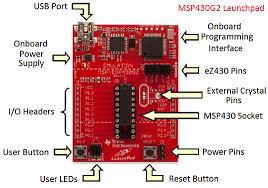
\includegraphics[scale=0.8]{board_msp430.jpeg}}
	\subfloat[fig:pindiagram][Pin Diagram]{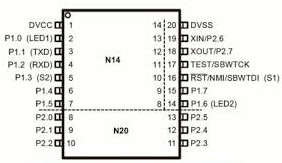
\includegraphics[scale=0.8]{pinout_msp430.jpeg}}
	\caption{Board details}
	\label{fig:board}
\end{figure}

\section{Interfacing Details}
      
MSP430 has an inbuilt Analog to Digital Converter abbreviated as ADC. The resolution of ADC is 10 bits. Analog to Digital converters functionally take in analog input and produce digital bits as outputs. Since the resolution is 10 bits, the number of levels during quantisation would be 1024. Here the task was to configure the LED outputs such that LEDs turned on based on analog input level. For demonstration purpose, the output range was divided into 2 parts and LED was turned on if the input signal exceeded that level and turned off otherwise. The challenge here was to enable a GPIO pin to sense the change in analog value and the controller would process the change and give a digital value. The result could be shown on the LEDs.

Digital to Analog converters abbreviated as DAC are used to convert back the digital signals after processing to analog so that this output signal analog in nature can be used for actuation. MSP430 unfortunately does not have an inbuilt DAC, hence an external DAC in form of a digital chip was employed. A digital input was fed to the 8 pins of the IC in form of high or low and this was converted into analog voltage at the output and this varying voltage was used to actuate or control the brightness of LED.


\subsection{General layout}
A few specifications for the DAC IC DAC0808 from Texas Instruments are listed in the form of a figure. Refer Figure \ref{fig:specs} above:
\begin{figure}[t]
	\centering
	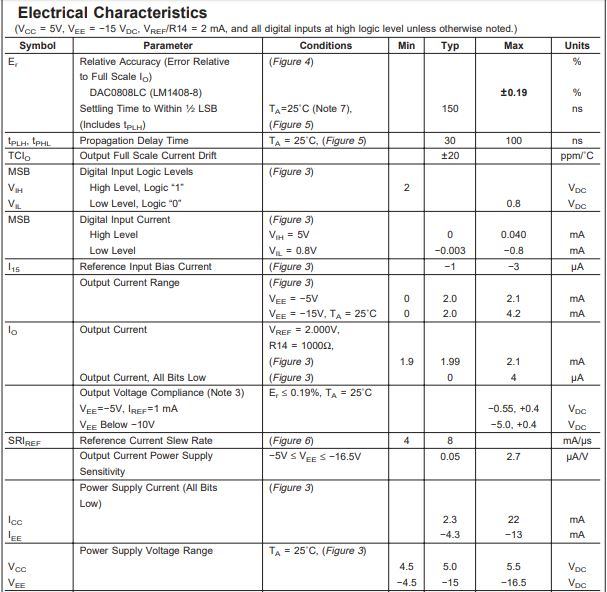
\includegraphics[scale=0.75]{Datasheet_DAC0808.JPG}
	\caption{Specifications in Datasheet}
	\label{fig:specs}
\end{figure}

\subsection{DAC0808}

The DAC0808 is an 8-bit monolithic digital-to-analog converter (DAC) featuring a full scale output current settling time of 150 ns while dissipating only 33 mW with ±5V supplies. No reference current (IREF) trimming is required for most applications since the full scale output current is typically ±1 LSB of 255 IREF/256. Relative accuracies of better than 0.19\% assure 8-bit monotonicity and linearity while zero level output current of less than 4 µA provides 8-bit zero accuracy for IREF greater than or equal to 2 mA. The power supply currents of the DAC0808 is independent of bit codes, and exhibits essentially constant device characteristics over the entire supply voltage range. The circuit used for interfacing is shown in Figure \ref{fig:DAC}.

\begin{figure}[t]
	\centering
	\subfloat[fig:DAC0808IC][DAC0808 IC]{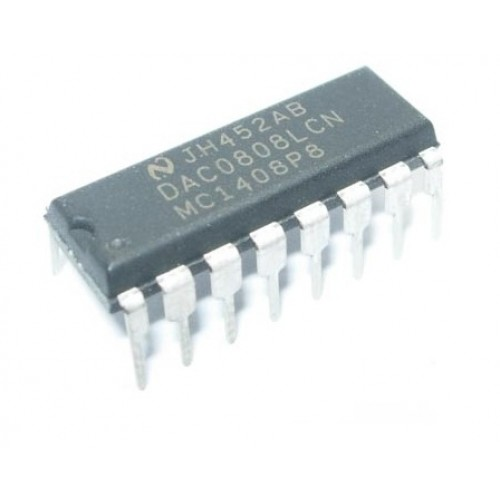
\includegraphics[scale=0.2]{DACIC.jpg}}
	\subfloat[fig:Circuit][Interfacing Circuit]{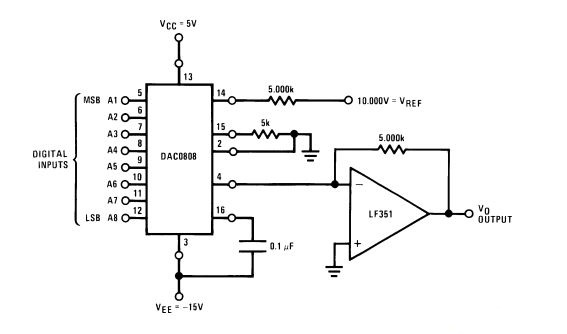
\includegraphics[scale=0.8]{Circuit_Diagram_DAC.JPG}}
	\caption{DAC0808 Interfacing Circuit}
	\label{fig:DAC}
\end{figure}


\section{Program}

The code for interfacing MSP430 with ADC and DAC are as follows:

%\begin{center}
\begin{longtable}{|p{8cm}||p{6cm}|}
%\caption{A sample long table.} \label{tab:long} \\

\hline 
\multicolumn{1}{|c|}{\textbf{Interfacing ADC using MSP430}} & \multicolumn{1}{c|}{\textbf{Pseudo code}}  \\ 

\hline 
\endfirsthead

\multicolumn{2}{c}%
{{\bfseries \tablename\ \thetable{} -- continued from previous page}} \\
\hline 
%\multicolumn{1}{|c|}{\textbf{First column}} & \multicolumn{1}{c|}{\textbf{Second column}} & \multicolumn{1}{c|}{\textbf{Third column}} \\ 
\hline 
\endhead

\hline \multicolumn{2}{|r|}{{Continued on next page}} \\ \hline
\endfoot

\hline \hline
\endlastfoot



\#include <msp430.h>  & \\             
unsigned int ADC\_value = 0; & \\
void adc\_setup(void) & \\
\{ & \\
\hspace{0.1cm}	ADC10CTL1 |$=$ INCH\_3; 	&  Channel 3\\
\hspace{0.1cm}	ADC10CTL0 |$=$ SREF\_0 + ADC10ON + ADC10SHT\_3; & VDD and VCC as reference, switch on ADC, Sample and Hold for 64 cycles \\
\hspace{0.1cm}	ADC10AE0 |$=$ BIT3;				&			 ADC input at P1.3\\
\} & \\
&\\
int main(void)\{ & \\

   \hspace{0.1cm} WDTCTL $=$  WDTPW $|$ WDTHOLD;    & Stop watchdog timer \\ 

    
  \hspace{0.1cm}   P1SEL |= BIT3;	& Select alternative function for P1.3 \\ 
  \hspace{0.1cm}   adc\_setup();	& Setup the ADC \\    
   \hspace{0.1cm} P1DIR = 0xF7; & Setting rest 7 pins to output\\
    \hspace{0.1cm} while(1) & \\
	\hspace{0.1cm}\{ & \\
   
     \hspace{0.3cm}   \_\_delay\_cycles(1000);	& Wait for ADC Ref to settle \\
     \hspace{0.3cm}   ADC10CTL0 |= ENC + ADC10SC;	& Sampling and conversion start\\
   \hspace{0.1cm} & \\
      \hspace{0.3cm}  \_\_bis\_SR\_register(CPUOFF + GIE);& Low Power Mode 0 with interrupts enabled \\
\hspace{0.1cm} & \\
      \hspace{0.3cm}   ADC\_value = ADC10MEM;& Assigns the value held in ADC10MEM to the integer called ADC\_value \\
      \hspace{0.1cm} & \\
      \hspace{0.3cm} if(ADC\_value > 512) & If the analog value is more than 512\\
        \hspace{0.5cm}     P1OUT = 0x01; & Turn on the External Led\\ 
        \hspace{0.3cm} else & If analog value is less than 512\\
        \hspace{0.5cm}    P1OUT = 0x00;; & Turn off the External Led\\
        \hspace{0.1cm} \} & \\

            \} & \\

\end{longtable}
%\end{center}



%\begin{center}
\begin{longtable}{|p{8cm}||p{6cm}|}
%\caption{A sample long table.} \label{tab:long} \\

\hline 
\multicolumn{1}{|c|}{\textbf{Interfacing DAC using MSP430}} & \multicolumn{1}{c|}{\textbf{Pseudo code}}  \\ 

\hline 
\endfirsthead

\multicolumn{2}{c}%
{{\bfseries \tablename\ \thetable{} -- continued from previous page}} \\
\hline 
%\multicolumn{1}{|c|}{\textbf{First column}} & \multicolumn{1}{c|}{\textbf{Second column}} & \multicolumn{1}{c|}{\textbf{Third column}} \\ 
\hline 
\endhead

\hline \multicolumn{2}{|r|}{{Continued on next page}} \\ \hline
\endfoot

\hline \hline
\endlastfoot



\#include <msp430.h>  & \\             

int main(void)\{ & \\

   \hspace{0.1cm} WDTCTL $=$  WDTPW $|$ WDTHOLD;    & Stop watchdog timer \\ 

   \hspace{0.1cm} P1DIR = 0xFF; & Setting 8 pins to output to give input to 8 pins of DAC\\
   \hspace{0.1cm} unsigned int dac\_value $=$ 0x00; & Initializing DAC INPUT \\
    \hspace{0.1cm} while(1) & \\
	\hspace{0.1cm}\{ & \\
   
     \hspace{0.3cm}   \_\_delay\_cycles(100);	& Wait for DAC Ref to settle \\
       \hspace{0.1cm} & \\
     \hspace{0.3cm}   P1OUT = dac\_value	& Setting MSP430 output pins to DAC value\\
   \hspace{0.1cm} & \\
      \hspace{0.3cm}  \_\_delay\_cycles(10); & Delay Between change in DAC value\\
\hspace{0.1cm} & \\
      
      
      \hspace{0.3cm} if(dac\_value == 0xFF) & If DAC value has reached Max\\
        \hspace{0.5cm}     dac\_value = 0x00 & Reset DAC value\\ 
        \hspace{0.3cm} else & else\\
        \hspace{0.5cm}    dac\_value = dac\=value + 1;; & Increment DAC value to increase the brightness of External LED\\
        \hspace{0.1cm} \} & \\

            \} & \\

\end{longtable}
%\end{center}


\newpage

\section{Knowledge gained}

\begin{enumerate}
	\item Since ADC was inbuilt, we learnt how to interface something already inbuilt in the chip by manipulating suitable registers and making use of dual functionality of the GPIO pins
	
	\item Interfaced DAC IC with the microcontroller and controlled the brightness of the LED based on digital input fed form the controller 
	
	\item ADCs and DACs form an integral part of any real world systems to convert analog into digital and vice-versa and learning to interface them was an asset to us. All real world signals are analog in nature
	
	\item DAC was used externally and we had to refer to the data sheet for specifications hence our data-sheet comprehending capability develops due to this
\end{enumerate}

\end{document}
